%==============================================================================
%  CSE 406 — Security Lab Project #8
%  Port Scanning with OS Information / Version — FINAL REPORT
%
%  Compile:  pdflatex final_report.tex   (run twice for refs/ToC)
%==============================================================================
\documentclass[11pt,a4paper]{article}

%------------------------------------------------------------------ Geometry
\usepackage[margin=2.4cm,top=2.5cm,bottom=2.5cm]{geometry}

%---------------------------------------------------------------- Typography
\usepackage{mathptmx}                 % Times body + math
\usepackage[scaled=0.90]{helvet}      % Helvetica for headings/sans
\usepackage[T1]{fontenc}
\usepackage[utf8]{inputenc}
\usepackage{microtype}
\usepackage{parskip}
\setlength{\parskip}{5pt}

%-------------------------------------------------------- Tables / lists / fig
\usepackage{booktabs}
\usepackage{tabularx}
\usepackage{array}
\usepackage{ragged2e}
\usepackage{enumitem}
\setlist{nosep,leftmargin=1.4em}
\usepackage{float}
\usepackage{graphicx}
\usepackage{caption}

%------------------------------------------------------------------- Palette
% Red-based scheme. Accent = deep crimson used for headings, rules, table
% headers; a stronger pure red is reserved for genuine highlights.
\usepackage{xcolor}
\definecolor{ink}{RGB}{28,32,38}          % near-black body ink
\definecolor{accent}{RGB}{155,26,32}      % deep crimson (primary accent)
\definecolor{primary}{RGB}{155,26,32}     % alias used by the cover page
\definecolor{accentstrong}{RGB}{200,16,24}% stronger red for real emphasis
\definecolor{accentsoft}{RGB}{247,228,229}% pale red for table header fill
\definecolor{rule}{RGB}{209,213,219}      % hairline grey
\definecolor{codebg}{RGB}{248,246,246}    % subtle mono frame background
\color{ink}

%------------------------------------------------------ Captions (understated)
\captionsetup{labelfont={bf,sf,color=accent},textfont={small},labelsep=period,skip=6pt}

%------------------------------------------------- Section headings (clean, thin rule)
\usepackage{titlesec}
\titleformat{\section}
  {\sffamily\large\bfseries\color{accent}}
  {\thesection}{0.7em}{}[{\vspace{2pt}\color{rule}\titlerule[0.8pt]}]
\titleformat{\subsection}
  {\sffamily\normalsize\bfseries\color{ink}}
  {\thesubsection}{0.6em}{}
\titlespacing*{\section}{0pt}{16pt}{7pt}
\titlespacing*{\subsection}{0pt}{11pt}{4pt}

%--------------------------------------------------- Header / footer (minimal)
\usepackage{fancyhdr}
\usepackage{lastpage}
\pagestyle{fancy}\fancyhf{}
\renewcommand{\headrulewidth}{0.4pt}
\renewcommand{\headrule}{\hbox to\headwidth{\color{rule}\leaders\hrule height 0.4pt\hfill}}
\fancyhead[L]{\footnotesize\sffamily\color{accent}CSE 406 — Project \#8}
\fancyhead[R]{\footnotesize\sffamily\color{ink}Port Scanning \& OS Fingerprinting}
\fancyfoot[C]{\footnotesize\sffamily\color{ink}\thepage\ / \pageref{LastPage}}

%----------------------------------------------------- Log / code excerpt box
% A subtle single-tint monospace frame — used consistently for tool output.
% Content is VERBATIM (via listings) so backslashes, braces, underscores,
% and ? in console output render literally with no escaping.
\usepackage[most]{tcolorbox}
\tcbuselibrary{listings}
\newtcblisting{logbox}{
  breakable, enhanced, sharp corners,
  colback=codebg, colframe=rule, boxrule=0.5pt,
  left=8pt,right=8pt,top=6pt,bottom=6pt,
  listing only,
  listing options={
    basicstyle=\ttfamily\footnotesize\color{ink},
    breaklines=true, columns=fullflexible, keepspaces=true,
    aboveskip=0pt, belowskip=0pt}}

% Raw-log listing style: tiny wrapping monospace for the full-log appendix.
% \rawlog{<file>}{<caption>} inputs a complete sanitised log verbatim.
\lstdefinestyle{rawlog}{
  basicstyle=\ttfamily\fontsize{6.4}{7.4}\selectfont\color{ink},
  breaklines=true, breakatwhitespace=false,
  columns=fullflexible, keepspaces=true,
  showstringspaces=false, tabsize=2,
  frame=single, rulecolor=\color{rule}, framesep=4pt,
  backgroundcolor=\color{codebg},
  breakindent=0pt, postbreak=\mbox{\textcolor{rule}{$\hookrightarrow$}\space},
  xleftmargin=2pt, xrightmargin=2pt, aboveskip=6pt, belowskip=2pt}
\newcommand{\rawlog}[2]{%
  \needspace{4\baselineskip}%
  {\vspace{2pt}\noindent\sffamily\small\bfseries\color{accent}#2}\par\vspace{2pt}%
  \lstinputlisting[style=rawlog]{logs/#1}\par\vspace{4pt}}

% A restrained key-point callout — used sparingly (only for real highlights).
\newtcolorbox{keypoint}[1][Key point]{
  enhanced, sharp corners,
  colback=accentsoft, colframe=accent, boxrule=0pt,
  leftrule=2.5pt, left=9pt,right=9pt,top=6pt,bottom=6pt,
  fonttitle=\sffamily\bfseries\footnotesize\color{accent},
  title={#1}, coltitle=accent}

% Captioned figure PLACEHOLDER (team drops the real screenshot in later).
% Renders a clean framed box so the PDF compiles before images exist.
\newcommand{\shotplaceholder}[1]{%
  \begin{center}
  \setlength{\fboxrule}{0.6pt}\setlength{\fboxsep}{0pt}%
  \textcolor{rule}{\fbox{\parbox[c][2.4cm][c]{0.86\linewidth}{\centering
  \sffamily\footnotesize\color{accent}[\,SCREENSHOT\,]\\[2pt]
  \color{ink}\normalfont\footnotesize #1}}}%
  \end{center}}

\usepackage{tikz}
\usetikzlibrary{shapes.geometric,arrows.meta,positioning,calc,fit,backgrounds}
\usepackage[hidelinks]{hyperref}
\usepackage{needspace}   % keep a heading + first lines together on a page

% Strong inline highlight — a genuine emphasis, used sparingly.
\newcommand{\hl}[1]{\textbf{\color{accentstrong}#1}}

% Keep every section heading from landing on the last line of a page:
% reserve ~4 lines before each \section so the heading + opening text stay together.
\let\origsection\section
\renewcommand{\section}{\Needspace*{4\baselineskip}\origsection}

%------------------------------------------------------------- New column type
\newcolumntype{L}[1]{>{\RaggedRight\arraybackslash}p{#1}}

% Table header helper: pale accent fill + bold sans
\newcommand{\thh}[1]{\textbf{\sffamily #1}}
\usepackage{colortbl}
\newcommand{\hdrrow}{\rowcolor{accentsoft}}

\begin{document}

%==============================================================================
%  COVER PAGE
%==============================================================================
\begin{titlepage}
\thispagestyle{empty}
\centering
\vspace*{0.4cm}

% --- LOGO ---

\includegraphics[width=0.22\textwidth]{rsc/buet.png}\\[0.8cm]

% --- INSTITUTION ---
{\Large \textsc{Bangladesh University of Engineering and Technology}}\\[0.3cm]
{\large \textsc{Department of Computer Science and Engineering}}\\[0.4cm]
{\normalsize CSE 406 — Computer Security Lab \quad·\quad Semester January 2026}\\[1.6cm]

% --- TITLE BLOCK ---
{\color{primary}\rule{\linewidth}{1mm}}\\[0.55cm]
{\LARGE\bfseries\color{primary} Port Scanning with OS Fingerprinting}\\[0.5cm]
{\large\bfseries Project \#8 — Attack Tools Implementation}\\[0.5cm]
{\color{primary}\rule{\linewidth}{1mm}}\\[1.4cm]

% --- SUBTITLE ---
{\Large\bfseries Final Report \& Implementation Demo}\\[2.6cm]

\vfill

% --- TEAM + SUPERVISOR side by side ---
\begin{minipage}[t]{0.52\textwidth}
\centering
{\large\bfseries Submitted By}\\[0.5cm]
{\renewcommand{\arraystretch}{1.35}\normalsize
\begin{tabular}{rl}
\textbf{2105033} & Abhishek Roy\\
\textbf{2105032} & Nawriz Ahmed Turjo\\
\end{tabular}}
\end{minipage}%
\begin{minipage}[t]{0.48\textwidth}
\centering
{\large\bfseries Supervised By}\\[0.5cm]
{\large\bfseries Anwarul Bashir Shuaib}\\[0.15cm]
{\normalsize Lecturer}\\[0.05cm]
{\footnotesize Dept.\ of Computer Science \& Engineering, BUET}
\end{minipage}

\vspace{1.6cm}

% --- DATE ---
{\large \today}\\[0.4cm]
\end{titlepage}

%==============================================================================
%  ABSTRACT + MEMBER RESPONSIBILITIES  (front matter)
%==============================================================================
\setcounter{page}{1}

\section*{\sffamily\color{accent}Executive Summary}
\addcontentsline{toc}{section}{Executive Summary}

This report documents the final implementation of a complete, self-authored network
reconnaissance and exploitation toolkit for Project~\#8, together with a defensive
countermeasure that qualifies for the defense bonus. Every Ethernet frame, IPv4 packet,
and TCP segment is constructed and parsed by our own code; no ready-made tool
(Nmap, Scapy) performs any attack step. Npcap and \texttt{libpcap} are used only as raw
packet I/O.

The delivered system substantially \emph{exceeds} the week-11 Design Report. Three upgrade
layers landed after that submission: (i)~the OS-fingerprinting engine grew from a single
passive SYN/ACK feature table into a \textbf{seven-strategy probabilistic engine}
(RST analysis, IP-ID sequencing, TCP-timestamp clock recovery, ECN probing, invalid-flag
probing, an ICMP/UDP battery, and cross-layer banner correlation); (ii)~the exploit set
became a \textbf{dynamic, OS-aware battery} of five modules across FTP, HTTP, and SSH; and
(iii)~the defense grew into a \textbf{four-vector, cross-platform auto-quarantine engine}
with self-healing firewall rules.

The toolkit was verified on a heterogeneous testbed of five real operating systems
(Windows~11, Kali~Linux, Android, iPadOS/Darwin, and an embedded-Linux router), with
\textbf{68/68} automated tests passing. Fingerprint attribution ranged from 48\%–76\%
confidence — reported honestly as coarse OS tiers, never as false certainty — and the
active defense severed live attack chains mid-execution on both Windows Firewall and Linux
Netfilter.

%------------------------------------------------------ Member responsibilities
\section*{\sffamily\color{accent}Group Member Responsibilities}
\addcontentsline{toc}{section}{Group Member Responsibilities}

Per the project requirement, the table below states which member was responsible for each
part of the implementation. Both members jointly authored the reports and participated in
the multi-device empirical verification.

\renewcommand{\arraystretch}{1.3}
\noindent\begin{tabularx}{\textwidth}{@{}L{4.2cm} X@{}}
\toprule
\hdrrow \thh{Member} & \thh{Responsibility}\\
\midrule
\textbf{Abhishek Roy}\newline\small(2105033) &
Binary framing and raw packet I/O — the from-scratch Ethernet/IPv4/TCP builder and
parser, RFC~1071 Internet checksum, Npcap \texttt{ctypes} bindings, and ARP/interface
resolution via the Windows IP Helper API. The TCP~SYN half-open scanning engine and
port-state tracking. Core OS-fingerprinting heuristics and version-tier calibration.
The \textbf{HTTP directory-traversal} and \textbf{SSH weak-credential} exploit modules.\\
\addlinespace
\textbf{Nawriz Ahmed Turjo}\newline\small(2105032) &
Advanced fingerprinting and active stimulus probing — the SYN option-offering probe,
closed-port RST fallback, IP-ID / timestamp / ECN / ICMP-UDP strategies, and cross-layer
banner correlation. The service banner grabber. The \textbf{FTP exploit suite}
(anonymous login, write$\rightarrow$web-shell$\rightarrow$RCE, and bounce) with
\textbf{OS-aware payload selection}. The multi-vector active-defense engine and the
end-to-end attack orchestration.\\
\bottomrule
\end{tabularx}
\renewcommand{\arraystretch}{1.0}

\clearpage
{\hypersetup{linkcolor=ink}\tableofcontents}
\clearpage

%==============================================================================
%  BODY  — sections filled in subsequent edits
%==============================================================================

%============================================================ SECTION 1: INTRODUCTION
\section{Introduction \& Recap of the Design}

\subsection{The attack and its objective}
Network reconnaissance is the opening move of any intrusion: before an attacker can act,
they must learn which services a target exposes, what software versions run there, and
which operating system underpins them. Project~8 asks us to build this capability
(port scanning with OS information and version) entirely from scratch, crafting every frame,
packet, and segment in our own code.

Our toolkit carries out a full reconnaissance-to-exploitation chain in five phases:
(1)~raw TCP~SYN port scanning, (2)~service banner grabbing, (3)~probabilistic OS
fingerprinting, (4)~OS-aware payload selection, and (5)~a dynamic exploit battery,
paired with (6)~a defensive detector that recognizes the scan and can quarantine the
attacker in real time.

\subsection{What changed since the Design Report}
The week-11 Design Report proposed a functional but smaller system. During
implementation the project expanded across three distinct areas.
This report is organized around that progression: each core section compares the
originally planned behavior with the delivered implementation. The table
below summarizes the additions.

\renewcommand{\arraystretch}{1.12}
\noindent\begin{tabularx}{\textwidth}{@{}L{3.2cm} L{5.2cm} X@{}}
\toprule
\hdrrow \thh{Area} & \thh{Design Report (week 11)} & \thh{Delivered implementation}\\
\midrule
OS fingerprinting &
Single passive SYN/ACK feature table (TTL, window, MSS, WScale, SACK, timestamp, option order). &
\textbf{Seven-strategy probabilistic engine}: RST analysis, IP-ID sequencing,
timestamp-clock recovery, ECN probe, invalid-flag probe, ICMP/UDP battery, cross-layer
banner correlation, with confidence scoring and coarse version tiers.\\
\addlinespace[3pt]
Exploit suite &
Three fixed proof-of-concept exploits (FTP anon, SSH, HTTP). &
\textbf{Five OS-aware modules} with dynamic payload selection: FTP anonymous, FTP
write$\rightarrow$web-shell$\rightarrow$RCE, FTP bounce, HTTP traversal, and SSH
brute-force with quiet/loud post-exploitation.\\
\addlinespace[3pt]
Active defense &
Single fast sliding-window SYN detector; Windows-only \texttt{netsh} block. &
\textbf{Four-vector, cross-platform engine}: fast + slow windows, invalid-flag detection,
canary honeyport; \texttt{netsh} \emph{and} \texttt{iptables}; self-healing TTL release,
whitelist, and JSON incident logging.\\
\addlinespace[3pt]
Test topology &
One generic Windows victim. &
\textbf{Five real operating systems}: Windows~11, Kali~Linux, Android, iPadOS/Darwin,
embedded-Linux router.\\
\addlinespace[3pt]
Verification &
Manual observation. &
\textbf{68 automated tests} plus twelve archived empirical run logs.\\
\bottomrule
\end{tabularx}
\renewcommand{\arraystretch}{1.0}

\subsection{Lab topology}
\noindent
\begin{minipage}[t]{0.45\textwidth}
\vspace{0pt}
The verification testbed is a single isolated private LAN. The attacker is a Windows~11 laptop running the toolkit over an Npcap adapter; the primary victim is a Windows~11 desktop hosting the vulnerable lab services; and a set of secondary targets on the same subnet exercises the fingerprinting engine against genuinely different TCP/IP stacks.

\vspace{3pt}
The attacker never leaves this private range: an RFC~1918 check refuses any non-private target, and the scanner is bounded (Section~\ref{sec:safety}) so that it cannot be repurposed as a flooding tool.
\end{minipage}\hfill
\begin{minipage}[t]{0.53\textwidth}
\vspace{0pt}
\centering
\resizebox{\linewidth}{!}{%
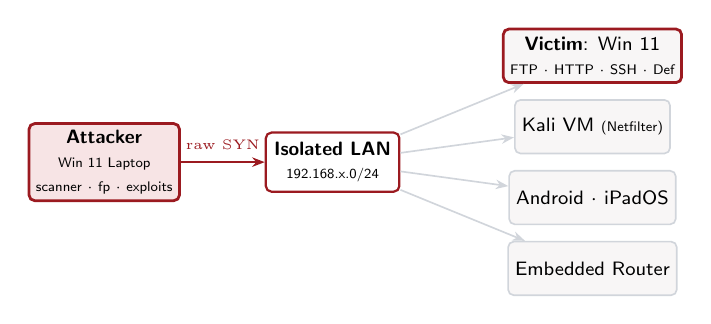
\begin{tikzpicture}[
  font=\sffamily\scriptsize, >={Stealth[length=1.6mm]},
  box/.style={rectangle, rounded corners=2pt, draw=rule, line width=0.6pt,
              fill=codebg, minimum height=0.68cm, align=center, inner sep=2.5pt},
  atk/.style={box, draw=accent, line width=1.0pt, fill=accentsoft},
  vic/.style={box, draw=accent, line width=1.0pt},
  hub/.style={rectangle, rounded corners=2pt, draw=accent, line width=0.8pt,
              fill=white, align=center, inner sep=3pt, minimum height=0.75cm}]

% attacker (left)
\node[atk] (atk) at (0,0) {\textbf{Attacker}\\[0.5pt]\tiny Win 11 Laptop\\[0.5pt]\tiny scanner $\cdot$ fp $\cdot$ exploits};

% LAN hub (centre)
\node[hub] (sw) at (2.9,0) {\textbf{Isolated LAN}\\[0.5pt]\tiny 192.168.x.0/24};

% targets (right column, compact)
\node[vic]  (vic)  at (6.2,1.35)  {\textbf{Victim}: Win 11\\[0.5pt]\tiny FTP $\cdot$ HTTP $\cdot$ SSH $\cdot$ Def};
\node[box] (kali) at (6.2,0.45)  {Kali VM \tiny(Netfilter)};
\node[box] (mob)  at (6.2,-0.45) {Android $\cdot$ iPadOS};
\node[box] (rtr)  at (6.2,-1.35) {Embedded Router};

% attacker -> hub
\draw[->,line width=0.8pt,accent] (atk) -- node[above=1pt,font=\tiny\color{accent}]{raw SYN} (sw);

% hub -> each target
\draw[->,line width=0.6pt,rule] (sw) -- (vic);
\draw[->,line width=0.6pt,rule] (sw) -- (kali);
\draw[->,line width=0.6pt,rule] (sw) -- (mob);
\draw[->,line width=0.6pt,rule] (sw) -- (rtr);
\end{tikzpicture}%
}
\vspace{-2pt}
\captionof{figure}{Heterogeneous verification testbed. One attacker drives probes across five distinct OS stacks on an isolated LAN.}
\label{fig:topology}
\end{minipage}

%========================================================= §2 IMPLEMENTATION
\section{Implementation: From-Scratch Packet Layer \& Architecture}

\subsection{Architecture and Software Module Map}
The toolkit is organized under \texttt{Imp/} as four modular, interacting packages: a low-level
shared packet layer, the offensive reconnaissance and exploitation engine, intentionally
vulnerable multi-platform lab services, and a host-based active defense countermeasure. The
delivered system layout is detailed in Table~\ref{tab:module_map}.

\begin{table}[htbp]
\centering
\small
\renewcommand{\arraystretch}{1.22}
\caption{Delivered Source Code Inventory and Component Responsibilities}
\label{tab:module_map}
\begin{tabularx}{\textwidth}{@{}L{4.4cm} X@{}}
\toprule
\hdrrow \thh{Module Path} & \thh{Engineering Role and Capabilities}\\
\midrule
\multicolumn{2}{@{}l}{\textit{\color{accent}\textbf{common/ — From-Scratch Binary Framing \& I/O Layer}}}\\
\texttt{packet.py} & Manual byte-by-byte serialization and parsing for Ethernet II, IPv4, TCP, ICMP, and UDP frames; RFC~1071 16-bit one's complement checksum engine.\\
\texttt{npcap.py} & Low-level \texttt{ctypes} bindings to Npcap and \texttt{libpcap}; packet injection, promiscuous capture, Windows IP Helper ARP resolution (\texttt{SendARP}), and adapter discovery.\\
\addlinespace
\multicolumn{2}{@{}l}{\textit{\color{accent}\textbf{attacker/ — Reconnaissance Orchestrator \& Heuristics}}}\\
\texttt{main.py} & Central attack pipeline executing Phases 1--5; CLI options for rate limiting, adapter binding, and exploit skipping.\\
\texttt{scanner.py} & Phase~1 raw Layer-2 TCP SYN half-open scanner; active diagnostic probe dispatch (ECN-SYN, SYN+FIN rule-breaker, ICMP, and UDP closed-port probes).\\
\texttt{fingerprint.py} & Phase~3 weighted probabilistic OS classification engine combining seven independent network stack heuristics.\\
\texttt{banner.py} & Phase~2 service banner grabber with protocol-aware probes (passive FTP greeting capture vs.\ active HTTP \texttt{HEAD} negotiation).\\
\addlinespace
\multicolumn{2}{@{}l}{\textit{\color{accent}\textbf{attacker/exploits/ — Dynamic, OS-Aware Exploit Battery}}}\\
\texttt{os\_payloads.py} & Phase~4 target adapter mapping OS-fingerprint tiers to targeted payloads (Windows \texttt{win.ini}/\texttt{whoami} vs.\ Linux \texttt{/etc/passwd}/\texttt{id}).\\
\texttt{ftp\_anon.py} & Exploit~1: RFC~959 unauthenticated anonymous login and passive directory listing (\texttt{PASV} + \texttt{LIST}).\\
\texttt{ftp\_web\_shell.py} & Exploit~2: Multi-stage FTP file write $\rightarrow$ web-shell upload $\rightarrow$ HTTP CGI RCE $\rightarrow$ automated forensic cleanup.\\
\texttt{ftp\_bounce.py} & Exploit~3: RFC~959 third-party \texttt{PORT} socket pivoting and host firewall mitigation reporting.\\
\texttt{http\_traversal.py} & Exploit~4: OS-aware unauthenticated directory traversal across canonical, backslash, and URL-encoded vectors.\\
\texttt{ssh\_bruteforce.py} & Exploit~5: Dictionary brute-force attack via bounded wordlist; quiet reconnaissance vs.\ loud multi-modal payload deployment.\\
\addlinespace
\multicolumn{2}{@{}l}{\textit{\color{accent}\textbf{defense/ — Active Host-Based Countermeasure Engine}}}\\
\texttt{detector.py} & Multi-vector inspection engine (fast sliding window, slow stealth window, decoy canary honeyports, and RFC~793 invalid flag traps).\\
\texttt{main.py} & Passive packet ingestion loop, cross-platform firewall mitigation (\texttt{netsh} and \texttt{iptables}), self-healing TTL daemon, and JSON SIEM logging.\\
\bottomrule
\end{tabularx}
\end{table}

\subsection{Binary Frame and Packet Construction Methodology}
A foundational requirement of Project~\#8 is that no off-the-shelf packet-crafting library (such
as Scapy or Nmap) may be utilized. Every network protocol data unit (PDU) dispatched by the
toolkit is manually packed byte-by-byte into raw binary buffers using Python's \texttt{struct}
module.

\subsubsection{Layer 2: Ethernet II Framing}
Because the scanner operates below the operating system's socket API, raw frames must include
a valid Layer-2 header. Each frame begins with a 14-octet Ethernet II header:
\begin{equation}
\text{Frame}_{\text{Eth}} = \langle \text{MAC}_{\text{dest}}\,(6\text{B}), \ \text{MAC}_{\text{src}}\,(6\text{B}), \ \text{EtherType} = \mathtt{0x0800}\,(2\text{B}) \rangle
\end{equation}

\begin{figure}[htbp]
\centering
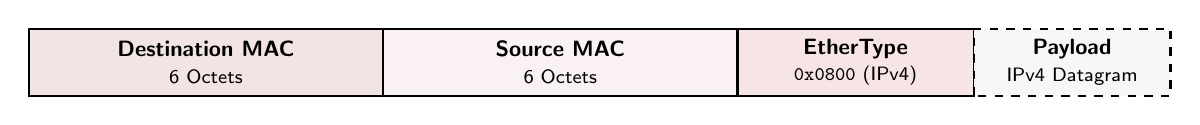
\begin{tikzpicture}[font=\sffamily\footnotesize]
    \draw[thick, fill=primary!12] (0, 0) rectangle (4.5, 0.85) node[midway, align=center] {\textbf{Destination MAC}\\\scriptsize 6 Octets};
    \draw[thick, fill=primary!6] (4.5, 0) rectangle (9.0, 0.85) node[midway, align=center] {\textbf{Source MAC}\\\scriptsize 6 Octets};
    \draw[thick, fill=accentsoft] (9.0, 0) rectangle (12.0, 0.85) node[midway, align=center] {\textbf{EtherType}\\\scriptsize \texttt{0x0800} (IPv4)};
    \draw[thick, fill=codebg, dashed] (12.0, 0) rectangle (14.5, 0.85) node[midway, align=center] {\textbf{Payload}\\\scriptsize IPv4 Datagram};
\end{tikzpicture}
\caption{Layer 2 Ethernet II Frame Structure (Total Header: 14 Octets).}
\label{fig:frame_eth}
\end{figure}

\subsubsection{Layer 3: IPv4 Packet Construction}
The Layer-3 IPv4 datagram is built in accordance with RFC~791. Standard probes utilize a 20-octet
base header without IP options. The fields are packed in big-endian network byte order
(\texttt{!BBHHHBBH4s4s}):
\begin{itemize}
    \item \textbf{Version \& IHL (1 byte):} Version 4 with Internet Header Length of 5 (20 octets), represented as \texttt{0x45}.
    \item \textbf{DSCP \& ECN (1 byte):} Default \texttt{0x00} for standard probes; modified during active RFC~3168 ECN probing.
    \item \textbf{Total Length (2 bytes):} Length of IPv4 header plus TCP segment (40 octets for bare SYN, 60 octets with options).
    \item \textbf{Identification (2 bytes):} Ephemeral 16-bit integer, initialized randomly per probe batch.
    \item \textbf{Flags \& Fragment Offset (2 bytes):} Don't-Fragment (DF) bit set (\texttt{0x4000}) with fragment offset zero.
    \item \textbf{Time to Live (TTL) (1 byte):} Outbound TTL set to 64 for scanner probes.
    \item \textbf{Protocol (1 byte):} Assigned to 6 (\texttt{IPPROTO\_TCP}) or 1 (\texttt{IPPROTO\_ICMP}).
    \item \textbf{Header Checksum (2 bytes):} Pre-computed over the 20-octet header with the checksum field initialized to 0.
    \item \textbf{Source and Destination IP (4 bytes each):} Packed 32-bit IPv4 addresses converted with Python's \texttt{inet\_aton()} socket call.
\end{itemize}

\begin{figure}[htbp]
\centering
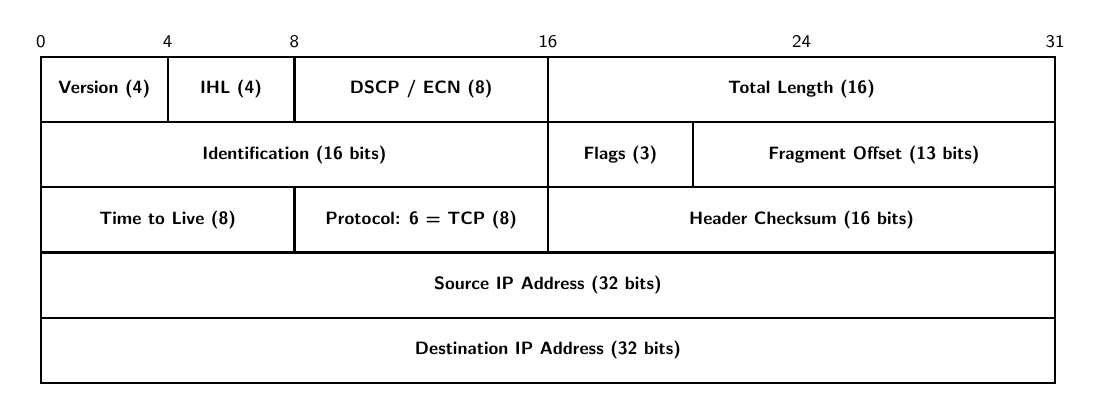
\begin{tikzpicture}[scale=0.92, every node/.style={transform shape}, font=\sffamily\scriptsize]
    \draw[thick] (0, 4.5) rectangle (14, 0);
    \node[above] at (0, 4.5) {0}; \node[above] at (1.75, 4.5) {4}; \node[above] at (3.5, 4.5) {8};
    \node[above] at (7.0, 4.5) {16}; \node[above] at (10.5, 4.5) {24}; \node[above] at (14, 4.5) {31};

    \draw[thick] (0, 3.6) -- (14, 3.6);
    \draw[thick] (1.75, 4.5) -- (1.75, 3.6); \draw[thick] (3.5, 4.5) -- (3.5, 3.6); \draw[thick] (7.0, 4.5) -- (7.0, 3.6);
    \node at (0.875, 4.05) {\textbf{Version (4)}}; \node at (2.625, 4.05) {\textbf{IHL (4)}};
    \node at (5.25, 4.05) {\textbf{DSCP / ECN (8)}}; \node at (10.5, 4.05) {\textbf{Total Length (16)}};

    \draw[thick] (0, 2.7) -- (14, 2.7);
    \draw[thick] (7.0, 3.6) -- (7.0, 2.7); \draw[thick] (9.0, 3.6) -- (9.0, 2.7);
    \node at (3.5, 3.15) {\textbf{Identification (16 bits)}};
    \node at (8.0, 3.15) {\textbf{Flags (3)}}; \node at (11.5, 3.15) {\textbf{Fragment Offset (13 bits)}};

    \draw[thick] (0, 1.8) -- (14, 1.8);
    \draw[thick] (3.5, 2.7) -- (3.5, 1.8); \draw[thick] (7.0, 2.7) -- (7.0, 1.8);
    \node at (1.75, 2.25) {\textbf{Time to Live (8)}};
    \node at (5.25, 2.25) {\textbf{Protocol: 6 = TCP (8)}};
    \node at (10.5, 2.25) {\textbf{Header Checksum (16 bits)}};

    \draw[thick] (0, 0.9) -- (14, 0.9);
    \node at (7.0, 1.35) {\textbf{Source IP Address (32 bits)}};
    \node at (7.0, 0.45) {\textbf{Destination IP Address (32 bits)}};
\end{tikzpicture}
\caption{Layer 3 IPv4 Packet Header Bit Layout (RFC 791, 20 Octets Base).}
\label{fig:header_ipv4}
\end{figure}

\subsubsection{Layer 4: TCP Header \& Active Diagnostic Option Offering}
The TCP segment header conforms to RFC~793. For a bare SYN frame, the base header is 20 octets
($\text{Data Offset} = 5$). However, sending bare SYN probes causes modern operating systems to
suppress advanced protocol capabilities in their SYN/ACK replies. To provoke maximum diagnostic
telemetry for OS fingerprinting, our probe engine formulates a 40-octet frame containing 20
octets of active option offerings (\texttt{STANDARD\_SYN\_OPTIONS}):
\begin{equation}
\text{Options}_{\text{SYN}} = \langle \text{MSS}(1460), \ \text{SACK\_Permitted}, \ \text{Timestamp}(t_0, 0), \ \text{NOP}, \ \text{WScale}(8) \rangle
\end{equation}
Offering these capabilities prompts target operating systems to reveal their compile-time option
ordering, native window scale factors, and timestamp clock frequencies in the return frame.

\begin{figure}[htbp]
\centering
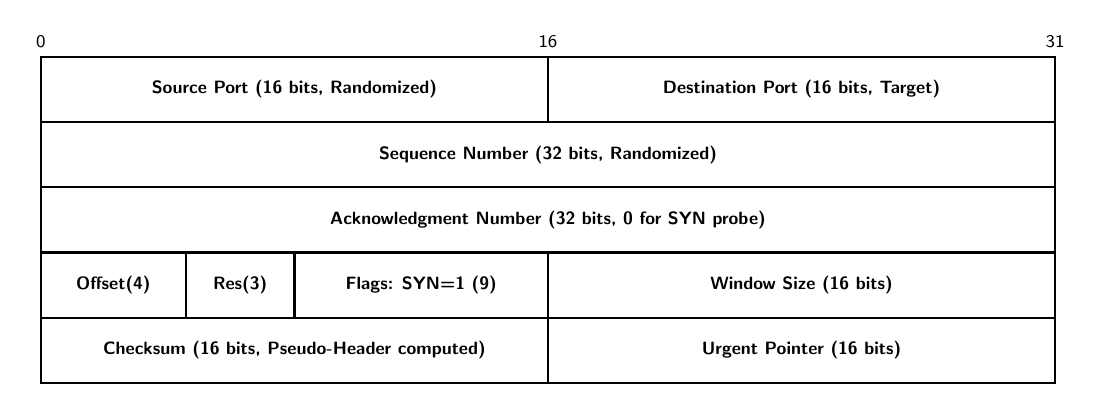
\begin{tikzpicture}[scale=0.92, every node/.style={transform shape}, font=\sffamily\scriptsize]
    \draw[thick] (0, 4.5) rectangle (14, 0);
    \node[above] at (0, 4.5) {0}; \node[above] at (7.0, 4.5) {16}; \node[above] at (14, 4.5) {31};

    \draw[thick] (0, 3.6) -- (14, 3.6); \draw[thick] (7.0, 4.5) -- (7.0, 3.6);
    \node at (3.5, 4.05) {\textbf{Source Port (16 bits, Randomized)}};
    \node at (10.5, 4.05) {\textbf{Destination Port (16 bits, Target)}};

    \draw[thick] (0, 2.7) -- (14, 2.7);
    \node at (7.0, 3.15) {\textbf{Sequence Number (32 bits, Randomized)}};

    \draw[thick] (0, 1.8) -- (14, 1.8);
    \node at (7.0, 2.25) {\textbf{Acknowledgment Number (32 bits, 0 for SYN probe)}};

    \draw[thick] (0, 0.9) -- (14, 0.9);
    \draw[thick] (2.0, 1.8) -- (2.0, 0.9); \draw[thick] (3.5, 1.8) -- (3.5, 0.9); \draw[thick] (7.0, 1.8) -- (7.0, 0.9);
    \node at (1.0, 1.35) {\textbf{Offset(4)}}; \node at (2.75, 1.35) {\textbf{Res(3)}};
    \node at (5.25, 1.35) {\textbf{Flags: SYN=1 (9)}}; \node at (10.5, 1.35) {\textbf{Window Size (16 bits)}};

    \draw[thick] (7.0, 0.9) -- (7.0, 0);
    \node at (3.5, 0.45) {\textbf{Checksum (16 bits, Pseudo-Header computed)}};
    \node at (10.5, 0.45) {\textbf{Urgent Pointer (16 bits)}};
\end{tikzpicture}
\caption{Layer 4 TCP Segment Header Bit Layout (RFC 793, 20 Octets Base).}
\label{fig:header_tcp}
\end{figure}

\subsection{RFC 1071 Checksum Computation \& Pseudo-Header Layout}
Both IPv4 header checksums and TCP segment checksums are computed using our self-authored 16-bit
one's complement algorithm. For TCP, RFC~793 requires prepending a 12-byte IPv4 pseudo-header
to ensure that packets delivered to the wrong host or protocol handler are discarded:
\begin{equation}
\text{Checksum} = \sim \left( \sum_{i=1}^{N} W_i \pmod{2^{16} - 1} \right)
\end{equation}
where $W_i$ denotes consecutive 16-bit binary words across the concatenated pseudo-header and TCP
segment. If the payload length is odd, a null padding octet is appended before summation.

\begin{table}[htbp]
\centering
\small
\renewcommand{\arraystretch}{1.2}
\caption{IPv4 TCP Pseudo-Header Field Layout for Checksum Computation}
\label{tab:pseudo_header}
\begin{tabularx}{\textwidth}{@{}L{2.8cm} L{4.6cm} X@{}}
\toprule
\hdrrow \thh{Byte Offset} & \thh{Field Designation} & \thh{Value Packed in Probe Frame}\\
\midrule
0--3   & Source IPv4 Address      & Bound local interface IP (e.g., \texttt{192.168.0.105})\\
4--7   & Destination IPv4 Address & Target host IP (e.g., \texttt{192.168.0.116})\\
8      & Reserved Octet           & \texttt{0x00}\\
9      & Protocol Identifier      & \texttt{0x06} (\texttt{IPPROTO\_TCP})\\
10--11 & TCP Segment Length       & Total octets of TCP header + options (e.g., 40 octets)\\
\bottomrule
\end{tabularx}
\end{table}

\subsection{Link-Layer Hardware Address Resolution Architecture}
Because standard Windows networking APIs do not expose raw Layer-2 interface bindings directly to
high-level scripts, our toolkit interfaces directly with the native Windows IP Helper library
(\texttt{iphlpapi.dll}) via Python's \texttt{ctypes}:
\begin{enumerate}
    \item \textbf{Local Interface Discovery:} The scanner identifies the active outbound interface
    by creating a connected UDP test socket toward the target subnet and reading \texttt{getsockname()}.
    It then invokes \texttt{GetAdaptersInfo()} to extract the active adapter name, Npcap device GUID,
    and 6-octet hardware MAC address.
    \item \textbf{Pre-Flight Target ARP Resolution:} Prior to probe transmission, the engine
    executes the Windows \texttt{SendARP()} API (passing target IP and MAC output buffer). This
    populates the local ARP cache and retrieves the destination hardware address across the Layer-2
    broadcast domain.
\end{enumerate}
This architecture eliminates the need for hardcoded MAC addresses and allows the raw Ethernet
builder to operate transparently across heterogeneous physical or virtualized interfaces.

\subsection{Operational Safety Rails}\label{sec:safety}
To ensure the toolkit remains strictly an educational reconnaissance instrument and cannot be
misused as an aggressive denial-of-service tool, five non-bypassable safeguards are enforced:
\begin{itemize}
    \item \textbf{RFC~1918 Scope Validation:} Targets are verified via Python's \texttt{ipaddress}
    library; public or routable Internet addresses are rejected immediately.
    \item \textbf{Bounded Probing Horizon:} Probe volume is capped at $\text{MAX\_PROBES} = 50$
    ports per execution run, preventing subnet sweeps or port flooding.
    \item \textbf{Mandatory Rate Limiting:} An inter-probe transmission delay $\ge 0.2$\,s (default
    0.5\,s) is enforced between consecutive packet dispatches.
    \item \textbf{Ephemeral Randomization:} Outbound source ports and initial sequence numbers are
    randomized per probe to prevent state overlap or collision.
    \item \textbf{Reversible Countermeasures:} All active firewall blocks inject bounded TTLs and
    are automatically flushed upon process termination.
\end{itemize}

%========================================================= §3 ATTACK STEPS
\section{Attack Steps \& Execution}\label{sec:steps}

This section answers requirement~(a): the concrete steps of the attack, with the tool's
own output as evidence and captioned placeholders for the demonstration screenshots. The
whole chain is driven by one command, for example:

\begin{logbox}
python attacker/main.py --target 192.168.0.116 --ports 21 22 80 81 \
       --adapter "\Device\NPF_{...}"
\end{logbox}

\subsection{Phase 1 — TCP SYN port scanning}
The scanner sends a raw SYN to each target port and classifies the reply: a SYN/ACK means
\textsc{open} (and no ACK is returned, keeping the connection half-open); a RST means
\textsc{closed}; silence past the timeout means \textsc{filtered}. Every open/closed reply
is also retained as OS-fingerprint evidence.

\begin{logbox}
[PHASE 1] TCP SYN Port Scanning  ->  192.168.0.116
   21  OPEN                           TTL=128 WIN=65535
   80  OPEN                           TTL=128 WIN=65535
   22  NO RESPONSE / POSSIBLY FILTERED
   81  NO RESPONSE / POSSIBLY FILTERED
\end{logbox}

\shotplaceholder{Attacker console — Phase 1 SYN scan output showing OPEN / CLOSED /
FILTERED port states with TTL and window values.}

\subsection{Phase 2 — service banner grabbing}
For each open port the grabber opens a full TCP connection and reads the service's
identifying banner; for HTTP it sends a \texttt{HEAD} probe and parses the \texttt{Server}
header. Banners feed both the report and the cross-layer fingerprint stage.

\begin{logbox}
[PHASE 2] Service Banner Grabbing
   21  FTP   -> 220 LabFTP Server Ready
   80  HTTP  -> Server: VulnHTTP/1.0 (Lab Demo)
\end{logbox}

\subsection{Phase 3 — OS fingerprinting}
The retained response features are scored by the probabilistic engine, which emits a most
likely OS family, a confidence percentage, a coarse version tier, and the evidence behind
the score. The engine and its seven strategies are detailed in Section~\ref{sec:fp}; a
representative verdict:

\begin{logbox}
[PHASE 3] OS Fingerprinting
   Likely OS  : Windows family        Confidence : 62%
   Version    : Windows 10 / 11 tier
   Evidence   : TTL=128 | WIN=65535 | IP-ID strict-incremental [27057,27059,27062]
              : TCP timestamp clock ~1000 Hz | ECN ignored | Windows option order
\end{logbox}

\subsection{Phase 4 — OS-aware payload selection}
Before any exploit runs, \texttt{os\_payloads.py} adapts the payloads to the fingerprinted
OS: a Windows verdict selects \texttt{windows\textbackslash win.ini} and \texttt{whoami};
a Linux verdict selects \texttt{/etc/passwd} and \texttt{id}. This closes the loop between
reconnaissance and weaponisation — the same binary attacks a Windows and a Linux host
differently, automatically.

\subsection{Phase 5 — exploit battery}
Each applicable exploit then executes. The FTP suite and HTTP traversal are pure-socket;
SSH uses \texttt{paramiko} for key exchange only, with our own attack logic on top.

\begin{itemize}
\item \textbf{FTP anonymous login} — authenticates as \texttt{anonymous}, then
\texttt{PWD}/\texttt{LIST} to prove data access.
\item \textbf{FTP write $\rightarrow$ web-shell $\rightarrow$ RCE} — uploads
\texttt{shell.py} into the writable \texttt{uploads/} directory, requests
\texttt{/uploads/shell.py?cmd=whoami} over HTTP to execute it, then deletes the artefact.
\item \textbf{FTP bounce} — attempts a \texttt{PORT} pivot; on a modern host this is
correctly rejected (see Section~\ref{sec:results}).
\item \textbf{HTTP directory traversal} — reads the OS-selected sensitive file across
several encodings (\texttt{..\textbackslash}, \texttt{../}, URL-encoded).
\item \textbf{SSH weak credentials} — brute-forces a small bounded wordlist, then runs
silent recon (quiet mode) or drops desktop trophy files and a spoken alert (loud mode).
\end{itemize}

\begin{logbox}
[EXPLOIT] FTP Web-Shell RCE (port 21+80)
  Status : SUCCESS   whoami -> homed01\turjo   (artefact cleaned up)
[EXPLOIT] HTTP Directory Traversal (port 80)
  Status : SUCCESS   read windows\win.ini  ([fonts] Arial=arial.ttf ...)
[EXPLOIT] FTP Bounce (port 21)
  Status : MITIGATED  [WinError 10053] connection aborted by host WFP
\end{logbox}

\shotplaceholder{Attacker console — Phase 5 exploit battery: FTP anonymous listing,
web-shell RCE output, and HTTP traversal file contents.}

\shotplaceholder{Victim desktop (SSH loud mode) — the injected \texttt{HACKED.py} script
and the \texttt{.bak}/text trophy file left on the Desktop with the attacker's message.
(The spoken voice alert is triggered on the victim's speakers and cannot be shown in a
still image.)}

%========================================================= §4 FINGERPRINTING
\section{OS Fingerprinting Engine}\label{sec:fp}

The fingerprinting engine is the largest single upgrade over the Design Report and the
technical centrepiece of the project. Where the design proposed a single passive feature
table, the delivered engine combines seven independent strategies into one probabilistic
verdict.

\subsection{The scoring model}
The Design Report's fingerprinting was a static lookup table. The delivered engine keeps
that table as one input but wraps it in a \textbf{weighted probabilistic model}. Every
strategy~$k$ contributes a weight $w_{k,c}$ to each OS class
$c \in \{\text{Windows},\text{Linux},\text{macOS/BSD},\text{Net.\ device}\}$. The raw score
and the reported confidence are

\[
S(c) \;=\; \sum_{k} w_{k,c}(\text{observed feature}),
\qquad
\text{Confidence}(c) \;=\; \frac{S(c)}{\sum_{c'} S(c')}\times 100\%.
\]

The engine reports $\arg\max_c S(c)$, its confidence, and the evidence list behind it. It
is deliberately \hl{probabilistic, not deterministic}: when evidence is thin the top score
is low, and the verdict is a coarse OS \emph{tier} (``Windows 10/11 tier''), never a
fabricated exact build. The seven strategies below each define $w_{k,c}$.

\subsection{The seven strategies}

\paragraph{Idea 1 — RST (closed-port) fingerprinting.}
When no port is open, the engine falls back to the RST returned by a \emph{closed} port,
keyed on the initial TTL (the RST window is typically $0$):
\begin{center}\small
\begin{tabular}{@{}ll@{\hskip 1.4em}ll@{}}
\toprule
\thh{Initial TTL} & \thh{Class ($w$)} & \thh{Initial TTL} & \thh{Class ($w$)}\\
\midrule
128 & Windows ($+4.5$)      & 255 & Net.\ device ($+4.0$)\\
64  & Linux ($+2.5$), BSD ($+2.0$) & -- & --\\
\bottomrule
\end{tabular}
\end{center}
This gives \hl{zero-open-port attribution}: on our Kali VM, closed ports alone scored 76\%
Linux.

\paragraph{Idea 2 — IP-ID sequence archetypes.}
Over several probes the engine takes 16-bit modular deltas
$\;\Delta_i = (\mathrm{ID}_i - \mathrm{ID}_{i-1}) \bmod 2^{16}\;$
and classifies the sequence:
\begin{center}\small
\begin{tabular}{@{}lll@{}}
\toprule
\thh{Archetype} & \thh{Condition} & \thh{Class ($w$)}\\
\midrule
\texttt{ALL\_ZERO}           & $\forall i:\ \mathrm{ID}_i = 0$ (RFC 6864, DF set) & Linux ($+2.5$)\\
\texttt{STRICT\_INCREMENTAL} & $\forall i:\ 1 \le \Delta_i \le 10$               & Windows ($+2.5$)\\
\texttt{BROKEN\_INCREMENTAL} & $\forall i:\ 1 \le \Delta_i \le 1000$             & Windows ($+2.0$)\\
\texttt{RANDOM\_POSITIVE}    & wide/pseudo-random $\Delta_i$                     & Darwin/BSD ($+1.5$)\\
\texttt{CONSTANT\_NONZERO}   & $\forall i:\ \mathrm{ID}_i = k \neq 0$            & Net.\ device ($+2.5$)\\
\bottomrule
\end{tabular}
\end{center}
Observed: Windows~11 $\to$ strict-incremental \texttt{[27057,27059,27062]}; Android $\to$
all-zero; iPad $\to$ random-positive.

\paragraph{Idea 3 — TCP timestamp clock \& uptime.}
From two samples the engine recovers the kernel tick rate and estimates uptime:
\[
R \;=\; \frac{(\mathrm{TSval}_i - \mathrm{TSval}_{i-1}) \bmod 2^{32}}{t_i - t_{i-1}}\ \text{Hz},
\qquad
\text{uptime} \approx \frac{\mathrm{TSval}_{\text{latest}}}{R}.
\]
\begin{center}\small
\begin{tabular}{@{}lll@{}}
\toprule
\thh{Archetype} & \thh{Condition} & \thh{Class ($w$)}\\
\midrule
\texttt{HZ\_1000}      & $700 \le R \le 1400$   & Windows ($+2.0$), Linux ($+1.0$)\\
\texttt{HZ\_250}       & $180 \le R \le 350$    & Linux ($+2.5$)\\
\texttt{RANDOM\_OFFSET}& $\Delta\mathrm{TSval} > 10^{7}$ (RFC 7323) & macOS/BSD ($+2.5$)\\
\bottomrule
\end{tabular}
\end{center}
Observed: Windows $\approx$1000\,Hz; iPad randomised (Darwin PRNG).

\paragraph{Idea 4 — ECN probe (active).}
A crafted SYN with ECE+CWR set (flags $=\mathtt{0xC2}$) tests RFC~3168 support by how the
reply's ECE bit comes back:
\begin{itemize}
\item \texttt{ECN\_SUPPORTED} — reply $\mathtt{0x52}$ (ECE reflected) $\Rightarrow$ Linux / macOS/BSD ($+2.0$).
\item \texttt{ECN\_IGNORED} — reply $\mathtt{0x12}$ (ECE cleared) $\Rightarrow$ default Windows stack ($+2.0$).
\item \texttt{ECN\_DROPPED} / \texttt{RST} — no ECN handshake $\Rightarrow$ network device.
\end{itemize}
Observed: Windows ignored ECN; Android and iPad supported it.

\paragraph{Idea 5 — invalid / ambiguous TCP flags (the ``rule-breaker'').}
RFC~793 does not define a reply to contradictory flags, so stacks diverge — a highly
discriminating signal:
\begin{center}\small
\begin{tabular}{@{}llll@{}}
\toprule
\thh{Probe} & \thh{Flags} & \thh{Windows} & \thh{Unix (Linux/BSD)}\\
\midrule
SYN+FIN & \texttt{0x03} & RST on open port & silently dropped\\
NULL    & \texttt{0x00} & RST               & dropped\\
XMAS    & \texttt{0x29} & RST               & dropped\\
\bottomrule
\end{tabular}
\end{center}
Notably, this is the \emph{same} behaviour our own defense engine watches for
(Section~\ref{sec:defense}).

\paragraph{Idea 6 — ICMP / UDP probing battery.}
Beyond TCP, an ICMP echo with a deliberately wrong code and a UDP probe to a closed port
expose further quirks:
\begin{itemize}
\item \textbf{ICMP code normalisation} — reply code $9\!\to\!0$ vs.\ reflected code~9.
\item \textbf{DF bit} in the echo reply, and shared TCP+ICMP IP-ID counter ($\Rightarrow$ Linux, $+3.0$).
\item \textbf{UDP unreachable quoting length} — Windows quotes exactly 8 bytes; Linux quotes more.
\end{itemize}
Because Windows Firewall often drops closed-TCP RSTs while still answering ICMP echo, this
battery is a valuable \hl{firewall-bypass fallback}.

\paragraph{Idea 7 / 7.1 — cross-layer banner correlation.}
Finally, Phase-2 banners feed the score as near-ground-truth evidence:
\begin{center}\small
\begin{tabular}{@{}ll@{}}
\toprule
\thh{Banner signature} & \thh{Attribution}\\
\midrule
\texttt{Microsoft-IIS}, Microsoft OpenSSH & Windows (very high)\\
\texttt{Apache/… (Ubuntu)}, Debian OpenSSH & Linux (very high)\\
\texttt{Server} before \texttt{Date} (RFC 7230 order) & weak corroboration\\
\bottomrule
\end{tabular}
\end{center}
When present, a banner is the single highest-confidence input the engine has.

\begin{keypoint}[Signal strength ranking]
\textbf{Strongest:} banner correlation and TCP option order (kernel-specific, hard to
spoof). \textbf{Strong:} invalid-flag probe and multi-sample IP-ID sequencing.
\textbf{Solid but ambiguous:} TTL (cannot split Linux from BSD alone).
\textbf{Corroborating:} ECN and the ICMP/UDP battery (middleboxes may alter them). The
engine's robustness comes from never trusting any single one in isolation.
\end{keypoint}

\subsection{Results across five operating systems}
The engine was run against every stack on the testbed. Confidence is reported honestly —
these are coarse-tier attributions, not exact-build claims.

\renewcommand{\arraystretch}{1.25}
\noindent\begin{tabularx}{\textwidth}{@{}L{3.4cm} L{3.0cm} X@{}}
\toprule
\hdrrow \thh{Target} & \thh{Verdict (confidence)} & \thh{Deciding evidence}\\
\midrule
Windows 11 desktop & Windows, 62--75\% & TTL 128; strict-incremental IP-ID; $\sim$1000\,Hz clock; ECN ignored; Windows option order.\\
Kali Linux VM & Linux, 66--76\% & TTL 64; all-zero IP-ID (RFC 6864); Debian OpenSSH/Apache banners; ECN supported.\\
Android 14 phone & Linux, 58\% & TTL 64; all-zero IP-ID with DF set; Linux option order.\\
Apple iPad (iPadOS 17) & macOS/BSD, 48\% & TTL 64; random-positive IP-ID; randomised timestamp offsets; Darwin option order (WScale before Timestamp).\\
Closed-port only (Kali) & Linux, 76\% & RST TTL 64; window 0; all-zero IP-ID; SYN+FIN silently dropped.\\
\bottomrule
\end{tabularx}
\renewcommand{\arraystretch}{1.0}

\noindent A fuller theoretical audit of every feature and its scoring weight is maintained
alongside the code in \texttt{fingerprint.md}.

%============================================================= SECTION 5: RESULTS
\section{Results \& Success Analysis}\label{sec:results}

This section answers requirement~(b): was the attack successful, and why or why not.

\subsection{Per-phase verdict}
\renewcommand{\arraystretch}{1.25}
\noindent\begin{tabularx}{\textwidth}{@{}L{4.2cm} L{2.6cm} X@{}}
\toprule
\hdrrow \thh{Phase / exploit} & \thh{Outcome} & \thh{Evidence}\\
\midrule
SYN port scan & \textbf{Success} & Open/closed/filtered states matched \texttt{netstat} on the victim; 100-port scale run classified all ports correctly.\\
Banner grabbing & \textbf{Success} & LabFTP, VulnHTTP, Apache, and Microsoft/Debian OpenSSH banners extracted.\\
OS fingerprinting & \textbf{Success$^\ast$} & Correct OS \emph{family} on all five stacks; confidence 48--76\% ($^\ast$probabilistic — see below).\\
FTP anonymous login & \textbf{Success} & \texttt{230 Login successful}; \texttt{/pub} and \texttt{/uploads} listed.\\
FTP web-shell RCE & \textbf{Success} & \texttt{whoami} $\rightarrow$ \texttt{homed01\textbackslash turjo}; artefact deleted.\\
HTTP traversal & \textbf{Success} & \texttt{win.ini} / \texttt{/etc/passwd} read across encodings.\\
SSH weak credentials & \textbf{Success} & Cracked \texttt{test:test123}; remote recon and payload drop executed.\\
FTP bounce & \textbf{Mitigated} & Rejected by the host stack — a correct, expected negative result (below).\\
\bottomrule
\end{tabularx}
\renewcommand{\arraystretch}{1.0}

\subsection{Why the attack succeeded}
Three properties made the chain effective. First, the \textbf{from-scratch packet layer is
correct}: because we parse the raw response ourselves, the fingerprint reads true stack
behaviour rather than library-normalised values, and the scanner's port classification
matched the victim's ground truth on every run. Second, the \textbf{fingerprint is robust
by combining many weak signals} — no single feature has to be decisive, so an altered TTL
or a suppressed timestamp does not derail the verdict. Third, and most importantly, the
\textbf{OS-aware payload stage closes the recon-to-exploitation loop}: the same binary read
\texttt{win.ini} on Windows and \texttt{/etc/passwd} on Linux automatically, which is why
the cross-platform run succeeded on both hosts without manual retargeting.

\subsection{Where it did not succeed — and why that is correct}
Two outcomes are deliberately \emph{not} full successes, and both are informative rather
than defects.

\begin{itemize}
\item \textbf{FTP bounce was mitigated.} The pivot was rejected by the Windows host with
\texttt{[WinError 10053]} — the modern kernel / Windows Filtering Platform refuses
unauthorised third-party \texttt{PORT} connections. Our tool correctly \emph{detected and
reported} the mitigation rather than failing silently, which is the right behaviour for a
reconnaissance tool.
\item \textbf{Fingerprinting is probabilistic, not certain.} Confidence sat at 48--76\%,
not 100\%. This is honest by design: TTL~64 cannot by itself separate Linux from macOS/BSD,
NAT and firewalls can alter fields, and a low-open-port target offers less evidence. We
report coarse OS tiers with their confidence rather than a fabricated exact build — a
deliberate accuracy choice, not a limitation we hide.
\end{itemize}

%============================================================= §6 OBSERVED
\section{Observed Output Across Machines \& Empirical Verification Matrix}

Requirement~(c) asks what was observed on each machine involved in the reconnaissance and attack
pipeline. Because our toolkit operates as a command-line reconnaissance and exploitation engine
whose primary outputs are structured terminal telemetry, the verbatim console records below
represent the decisive artifacts of system behavior across both offensive and defensive roles.

\subsection{Attacker Workstation Observations}
On the attacking machine (\texttt{192.168.0.105}), the console provides real-time visibility into
each attack phase:
\begin{enumerate}
    \item \textbf{Phase 1 (SYN Half-Open Scan):} Displays instantaneous port classification
    (\textsc{open}, \textsc{closed}, \textsc{filtered}) alongside the extracted initial TTL and
    TCP Window Size.
    \item \textbf{Phase 2 (Banner Grabbing):} Prints extracted service strings and daemon version
    metadata.
    \item \textbf{Phase 3 (OS Fingerprinting):} Displays the probabilistic verdict, confidence tier,
    and a bulleted breakdown of supporting evidence.
    \item \textbf{Phase 4 \& 5 (Weaponization \& Exploitation):} Reports payload dispatch status,
    exfiltrated file previews, and remote code execution outputs.
    \item \textbf{Severance Observation (Defense Run):} When active defense is enabled on the victim,
    the attacker console observes connection timeouts (\texttt{WinError 10060}) mid-execution once
    firewall quarantine rules take effect.
\end{enumerate}

\subsection{Victim Server Daemon Logs}
The victim machine hosts the vulnerable lab services (\texttt{victim/http\_server.py} on port~80 and
\texttt{victim/ftp\_server.py} on port~21). The service logs below record the corresponding inbound
exploit interactions from the server's perspective:

\begin{logbox}
[Victim Terminal 1: HTTP Server (Port 80)]
[HTTP] Vulnerable HTTP server listening on 0.0.0.0:80 (CGI enabled for uploads/*.py)
[HTTP] ('192.168.0.105', 51482) -> HEAD /
[HTTP] ('192.168.0.105', 51488) -> GET /uploads/shell.py?cmd=whoami
[HTTP] ('192.168.0.105', 51488) -> CGI executed shell.py (query='cmd=whoami')
[HTTP] ('192.168.0.105', 51493) -> GET /..\..\..\..\..\windows\win.ini  (200 OK, served)
[HTTP] ('192.168.0.105', 51498) -> GET /..%5c..%5c..%5cwindows%5cwin.ini (200 OK, served)

[Victim Terminal 2: FTP Server (Port 21)]
[FTP] Vulnerable FTP server listening on 0.0.0.0:21
[FTP] 220 LabFTP Server Ready
[FTP] USER anonymous -> 331 Password required
[FTP] PASS anon@lab -> 230 Login successful
[FTP] PASV -> 227 Entering Passive Mode (192,168,0,116,195,84)
[FTP] LIST -> 150 Here comes the directory listing
[FTP] STOR uploads/shell.py -> 226 Transfer complete
[FTP] DELE uploads/shell.py -> 250 File deleted successfully (Forensic cleanup)
\end{logbox}

\subsection{Master Summary Matrix of Empirical Verification Runs}
Table~\ref{tab:master_matrix} summarizes the definitive empirical verification runs archived in
\texttt{final-log/}, cross-referencing target platforms, tested services, and observed defense states.

\begin{table}[htbp]
\centering
\footnotesize
\renewcommand{\arraystretch}{1.18}
\caption{Consolidated Master Matrix of Empirical Verification Test Runs}
\label{tab:master_matrix}
\begin{tabularx}{\textwidth}{@{}L{2.8cm} L{2.6cm} L{3.0cm} L{2.2cm} X@{}}
\toprule
\hdrrow \thh{Log Name} & \thh{Target System} & \thh{Tested Ports \& States} & \thh{Defense State} & \thh{Attribution \& Outcome}\\
\midrule
\texttt{full-chain.log} & Windows 11 Desktop & 21, 80 (Open), 22, 81 (Filtered) & Active Blocker On & Windows 62\%; 3/4 exploits succeeded; severed on Run 2.\\
\addlinespace
\texttt{cross-platform.log} & Windows 11 + Kali 6.x & 21, 80 (Win) / 21, 22, 80 (Kali) & Passive / Off & Dynamic OS payload swap: \texttt{win.ini} vs.\ \texttt{/etc/passwd}.\\
\addlinespace
\texttt{kali.log} & Kali Linux VM & 22, 80, 81 (All Closed / RST) & Passive / Off & Linux 76\% (Closed-port RST) / 67\% (ICMP Code 9 fallback).\\
\addlinespace
\texttt{scan\_100\_ports.log} & Windows 10/11 Target & 100 ports (2 $\times$ 50 batches) & Passive / Off & Batch 1: Win 71\% (SYN/ACK); Batch 2: Win 69\% (RST).\\
\addlinespace
\texttt{ipad.log} & Apple iPad (iPadOS 17) & 80 (Open VLC), 8080 (Closed) & Passive / Off & macOS/BSD 48\% (Darwin option order, WScale=5).\\
\addlinespace
\texttt{phn.log} & Android 14 Smartphone & 2221 (Open FTP), 2122 (Closed) & Passive / Off & Linux 58\% (SACK before TS, RFC 6864 IP ID=0).\\
\addlinespace
\texttt{ssh\_attack.log} & Windows OpenSSH Host & 22 (Open SSH) & Passive / Off & Windows 75\%; cracked \texttt{test:test123}; loud desktop payloads.\\
\addlinespace
\texttt{defense\_win.log} & Windows 11 Desktop & Multi-port scan (Scenarios A--G) & Windows Firewall & Tripped at 8 SYNs; canary port 81; auto-release after 60s.\\
\addlinespace
\texttt{defense\_kali.log} & Kali Linux VM & Multi-port scan (Scenarios A--G) & Linux Netfilter & Netfilter \texttt{iptables} DROP counter climbing dynamically.\\
\bottomrule
\end{tabularx}
\end{table}

\subsection{Cross-Platform Operating System Comparison}
Table~\ref{tab:os_comparison} highlights the contrasting stack signatures observed between Microsoft
Windows and Unix-like targets across identical probe sequences:

\begin{table}[htbp]
\centering
\small
\renewcommand{\arraystretch}{1.2}
\caption{Cross-Platform Network Stack Behavioral Signatures Observed in Testbed}
\label{tab:os_comparison}
\begin{tabularx}{\textwidth}{@{}L{3.6cm} L{4.6cm} X@{}}
\toprule
\hdrrow \thh{Diagnostic Metric} & \thh{Windows 11 Desktop} & \thh{Kali Linux / Android}\\
\midrule
Initial IPv4 TTL & 128 & 64\\
TCP Window Size & 65535 or 8192 & 29200, 65160, or 0 (closed RST)\\
IP-ID Sequence Archetype & \texttt{STRICT\_INCREMENTAL} ($\Delta \approx 1\dots 3$) & \texttt{ALL\_ZERO} ($\mathrm{ID} = 0$, RFC 6864 DF=1)\\
TCP Timestamp Clock Rate & Calibrated $\approx 1000$\,Hz (1\,ms tick) & $\approx 250$\,Hz or 1000\,Hz\\
RFC 3168 ECN Negotiation & Ignored (\texttt{0x12} returned) & Supported (\texttt{0x52} ECE reflected)\\
Invalid Flag Probe (SYN+FIN) & Emits TCP RST on open port & Silently dropped without reply\\
ICMP Non-Standard Code 9 & Normalized to Code 0 & Reflected unaltered as Code 9\\
OS-Aware Traversal Target & \texttt{windows\textbackslash win.ini} & \texttt{/etc/passwd}\\
RCE Command Execution & \texttt{whoami} $\to$ \texttt{homed01\textbackslash turjo} & \texttt{id} $\to$ \texttt{uid=0(root)}\\
\bottomrule
\end{tabularx}
\end{table}

%===================================================== SECTION: EMPIRICAL SUITE
\section{Empirical Verification Suite}\label{sec:empirical}

Every claim in this report is backed by an archived run log under \texttt{final-log/}.
Twelve runs span five real operating systems, both defense platforms, a 100-port scale
test, and two SSH post-exploitation modes. Rather than summarise them, this section walks
the decisive runs and shows the \emph{actual tool output} — the real proof of the work.
Each excerpt is verbatim from the cited log.

\renewcommand{\arraystretch}{1.2}
\noindent\begin{tabularx}{\textwidth}{@{}L{4.4cm} L{2.3cm} X@{}}
\toprule
\hdrrow \thh{Log} & \thh{Target} & \thh{Demonstrates}\\
\midrule
{\small\texttt{full-chain.log}}        & Win 11 & Full 5-phase chain + live defense severing (\S\ref{sub:fullchain})\\
{\small\texttt{cross-platform-exploit.log}} & Win + Kali & OS-aware exploitation on two OSes (\S\ref{sub:crossplat})\\
{\small\texttt{kali.log}}              & Kali VM & Zero-open-port \& ICMP fingerprinting (\S\ref{sub:closed})\\
{\small\texttt{scan\_100\_ports.log}}  & Win 10/11 & 100-port scale test (\S\ref{sub:scale})\\
{\small\texttt{defense\_win\_test.log}}& Win 11 & Four-vector defense, \texttt{netsh} (\S\ref{sub:defwin})\\
{\small\texttt{defense\_kali\_test.log}}& Kali VM & Four-vector defense, \texttt{iptables} (\S\ref{sub:defkali})\\
{\small\texttt{ssh\_quiet/attack.log}} & Win 11 & SSH brute-force + post-exploitation (\S\ref{sub:ssh})\\
{\small\texttt{ipad.log}, \texttt{phn.log}} & iPad, Android & Darwin \& Linux fingerprints (\S\ref{sub:mobile})\\
\bottomrule
\end{tabularx}
\renewcommand{\arraystretch}{1.0}

%--------------------------------------------------------------------
\subsection{Flagship end-to-end run}\label{sub:fullchain}
\texttt{full-chain.log} drives the complete toolkit against the Windows~11 victim
(\texttt{192.168.0.116}). Phase~1 classifies each port from its raw reply:
\begin{logbox}
   21  OPEN                           TTL=128 WIN=65535
   22  NO RESPONSE / POSSIBLY FILTERED
   80  OPEN                           TTL=128 WIN=65535
   81  NO RESPONSE / POSSIBLY FILTERED
\end{logbox}

Phase~3 then scores the open-port SYN/ACK. Note the honest confidence (62\%) and the full
evidence trail — TTL, window, DF, the IP-ID sequence, and the exact TCP option order:
\begin{logbox}
  Candidate  : Open-Port TCP SYN/ACK
  Likely OS  : Windows          Confidence : 62%
  Version    : Windows 10 / 11 / Server 2016+
  TTL        : 128 (initial 128, ~0 hop(s))    Window : 65535    DF bit : set
  IP ID Seq  : [27057, 27059, 27062] (deltas: [2, 3])   IP ID Class: STRICT_INCREMENTAL
  Options    : ('MSS',1460),('NOP',),('WSCALE',8),('SACK_PERMITTED',),('TIMESTAMP',...)
\end{logbox}

Phase~5's chained FTP-write$\to$web-shell$\to$RCE exploit confirms remote code execution and
cleans up after itself:
\begin{logbox}
  Status  : SUCCESS
  Detail  : RCE confirmed via uploads/shell.py (command: whoami).
    OK login  OK write_check  OK upload  OK http_access  OK rce  OK cleanup (Deleted shell.py)
  RCE output:  Host OS : Windows 11   Executed : whoami
    homed01\turjo
\end{logbox}

The FTP bounce, by contrast, is correctly \hl{detected as mitigated} rather than failing
silently — the modern Windows stack aborts the third-party pivot:
\begin{logbox}
  Status  : FAILED
  Detail  : PORT command rejected or connection aborted
            (500 [WinError 10053] ...). FTP bounce is mitigated by host firewall.
    192.168.0.116:80 -> blocked
\end{logbox}

%--------------------------------------------------------------------
\subsection{OS-aware exploitation across two operating systems}\label{sub:crossplat}
\texttt{cross-platform-exploit.log} runs the \emph{identical} binary against Windows and
Kali back-to-back. The engine fingerprints each host and Phase~4 swaps the payloads
automatically — the clearest proof that reconnaissance drives weaponisation. The two hosts
fingerprint distinctly (Windows 62\% strict-incremental IP-ID; Linux 66\% all-zero IP-ID),
and the same code path produces OS-correct RCE on each:
\begin{logbox}
[WIN  192.168.0.116]  fingerprint -> Windows (62%)   IP ID Class: STRICT_INCREMENTAL
   payload : windows\win.ini + whoami
   RCE     : homed01\turjo
[KALI 192.168.56.101] fingerprint -> Linux (66%)     IP ID Class: ALL_ZERO
   payload : /etc/passwd + id
   RCE     : uid=0(root) gid=0(root) groups=0(root)
\end{logbox}

%--------------------------------------------------------------------
\subsection{Zero-open-port and ICMP fingerprinting}\label{sub:closed}
\texttt{kali.log} proves the engine still works when \emph{nothing is open}. With all three
probed ports closed, the closed-port RST path alone attributes the OS at 76\% — a fallback
the Design Report did not have:
\begin{logbox}
   22  CLOSED   TTL= 64 WIN=0     80  CLOSED   TTL= 64 WIN=0     81  CLOSED   TTL= 64 WIN=0

  Candidate  : Closed-Port TCP RST      Likely OS : Linux      Confidence : 76%
  TTL : 64      Window : 0      IP ID Class: ALL_ZERO
  Probability:  Linux 76%  ###############   macOS/BSD 24%  ####   Windows 0%
\end{logbox}

Under \texttt{--prefer-icmp}, the ICMP Echo Reply candidate independently confirms Linux at
67\% — a firewall-bypass path when closed-TCP RSTs are dropped but ICMP is answered.

%--------------------------------------------------------------------
\subsection{100-port scale test}\label{sub:scale}
\texttt{scan\_100\_ports.log} verifies the scanner at scale (two 50-port batches, honouring
\texttt{MAX\_PROBES}). Batch~1 finds the Windows RPC/SMB ports and fingerprints from the
SYN/ACK; Batch~2 (all closed) fingerprints from RST — both agree on Windows:
\begin{logbox}
   135 OPEN TTL=128 WIN=65535   139 OPEN TTL=128 WIN=8192
   445 OPEN TTL=128 WIN=65535   1025 OPEN TTL=128 WIN=65535

  Batch 1  Open-Port SYN/ACK  -> Windows 71%   (clock ~1001 Hz, uptime ~3d 5h)
  Batch 2  Closed-Port RST     -> Windows 69%   (IP ID STRICT_INCREMENTAL, WIN=0)
\end{logbox}

%--------------------------------------------------------------------
\subsection{Active defense on Windows Firewall}\label{sub:defwin}
\texttt{defense\_win\_test.log} exercises all four detection vectors on Windows, each
injecting a \texttt{netsh} block with a self-healing TTL. The fast-window vector trips on
the 8th SYN:
\begin{logbox}
[ALERT] 192.168.0.105 | fast port scan (SYN=8, distinct ports=8 within 10.0s)
[MITIGATION] Blocked TCP traffic from 192.168.0.105
             Firewall rule : CustomPortScanBlock_192_168_0_105 (Windows)
             Auto-release  : after 60s (self-healing)
\end{logbox}
The canary honeyport severs the attacker on the single packet that touches port~81, and the
invalid-flag vector catches the fingerprinter's own SYN+FIN probe instantly:
\begin{logbox}
[ALERT] 192.168.0.105 | hit canary honeyport (81)
[CRITICAL ALERT] 192.168.0.105 -> 192.168.0.116:21 |
        invalid TCP flag combination (SYN+FIN (Rule-Breaker), 0x03) on port 21
[MITIGATION] Released quarantine block on 192.168.0.105 (TTL 60s elapsed)
\end{logbox}
The slow/stealth vector separately caught a 2.5\,s-spaced scan at its 20th SYN. The injected
rule is the literal command \texttt{netsh advfirewall firewall add rule
name=CustomPortScanBlock\_192\_168\_0\_105 dir=in action=block remoteip=192.168.0.105
protocol=TCP profile=any}.

\paragraph{Live disruption (full-chain Run~2).}
With the defense active, the first exploit completed and every later stage timed out once
the rule landed — the attack chain was cut mid-execution:
\begin{logbox}
SYN 192.168.0.105 -> 192.168.0.116:55455  window_count=10  distinct_ports=5
[ALERT] Possible TCP port scan from 192.168.0.105
[MITIGATION] Blocked TCP traffic from 192.168.0.105
             Firewall rule: CustomPortScanBlock_192_168_0_105
  ... Exploit 2 -> Connection failed: timed out   traversal -> All 4 payloads failed ...
\end{logbox}

%--------------------------------------------------------------------
\subsection{Active defense on Linux Netfilter}\label{sub:defkali}
\texttt{defense\_kali\_test.log} mirrors every vector on Kali via
\texttt{iptables -I INPUT ... -j DROP}. The strongest Linux-specific evidence is the kernel
DROP counter climbing as the attacker's packets are dropped at the Netfilter layer:
\begin{logbox}
[ALERT] 192.168.56.1 | fast port scan (SYN=8, distinct ports=8 within 10.0s)
[MITIGATION] Firewall rule : CustomPortScanBlock_192_168_56_1 (Linux)
  iptables -L INPUT -n -v :
    12 pkts DROP tcp -- 192.168.56.1   ->   13 pkts   ->   14 pkts   ->   16 pkts
\end{logbox}

%--------------------------------------------------------------------
\subsection{SSH brute-force and post-exploitation}\label{sub:ssh}
Against a Windows OpenSSH host (\texttt{SSH-2.0-OpenSSH\_for\_Windows\_9.5}, fingerprinted
Windows 75\%), both SSH runs crack \texttt{test:test123} on attempt 15/20. Quiet mode stops
at recon; loud mode escalates to visible impact:
\begin{logbox}
  Status : SUCCESS   Logged in as test:test123 (attempt 15/20)
  whoami -> aisheepc\test   hostname -> AisheePC
  os_info -> Microsoft Windows [Version 10.0.26200.9445]
  [LOUD] desktop_proof  -> PROOF_OF_ACCESS.txt created on Desktop
  [LOUD] hacked_payloads-> HACKED.exe, HACKED.bat, hacked.py created on Desktop
  [LOUD] voice_alert    -> spooky voice alert played on victim speakers
\end{logbox}

%--------------------------------------------------------------------
\subsection{Mobile and BSD stacks}\label{sub:mobile}
The mobile targets confirm the engine generalises beyond desktop OSes. The iPad
(\texttt{ipad.log}) is attributed to macOS/BSD on its Darwin option order, and the Android
phone (\texttt{phn.log}) to Linux on its option layout and zero IP-ID:
\begin{logbox}
[iPad]    macOS / BSD 48%  options ['MSS','WSCALE','TIMESTAMP','SACK_PERMITTED'] (BSD layout)
[Android] Linux 58%        options ['MSS','SACK_PERMITTED','TIMESTAMP','WSCALE'] (Linux layout)
\end{logbox}

\begin{keypoint}[On honest reporting]
Two of the raw logs carry an over-optimistic ``99\%'' figure in a trailing prose summary,
but every actual fingerprint \emph{verdict block} reports 48--76\%. This report quotes only
the verdict blocks — the values the engine actually computes — never the inflated footer.
\end{keypoint}

\noindent The excerpts above are drawn from the twelve run logs, which are reproduced
\textbf{in full and verbatim in Appendix~C} — the complete, unedited proof of every claim in
this report.

%============================================================= §7 DEFENSE
\section{Countermeasure: Active Defense Engine}\label{sec:defense}

Requirement~(d) asks whether we designed a countermeasure and how. We did, and it is the
project's bonus deliverable: a host-based detector that recognises the scan in real time
and can quarantine the attacker automatically. It runs on the victim and treats our own
scanner as the adversary.

\subsection{From the designed detector to a multi-vector engine}
The Design Report proposed a single fast sliding-window SYN detector with a Windows-only
\texttt{netsh} block. The delivered engine keeps that as one vector and adds three more,
plus cross-platform mitigation and self-healing.

\renewcommand{\arraystretch}{1.25}
\noindent\begin{tabularx}{\textwidth}{@{}L{3.6cm} X@{}}
\toprule
\hdrrow \thh{Detection vector} & \thh{How it works}\\
\midrule
Fast SYN window & Alerts when one source sends $\geq$8 SYNs across $\geq$5 distinct ports within 10\,s. The dual count-and-diversity condition suppresses false positives from a busy legitimate client.\\
Slow / stealth window & A longer 60\,s window ($\geq$20 SYNs) catches low-and-slow scans that deliberately pace probes to evade the fast window.\\
Invalid-flag detection & Any NULL, FIN-only, XMAS, or SYN+FIN packet is flagged instantly — no legitimate traffic uses these, so one such packet is enough.\\
Canary honeyport & Any connection to a decoy port (default 81), which no real service uses, triggers instant quarantine — the attacker cannot know which ports are decoys.\\
\bottomrule
\end{tabularx}
\renewcommand{\arraystretch}{1.0}

\subsection{From detection to mitigation}
When \texttt{--block} is set, a detected attacker is quarantined by injecting a firewall
rule — \texttt{netsh advfirewall} on Windows or \texttt{iptables -I INPUT … -j DROP} on
Linux. Three properties make this safe to run live:

\begin{itemize}
\item \textbf{Idempotent.} An already-blocked IP is not re-blocked, so the flood of alerts
during a scan produces exactly one rule.
\item \textbf{Self-healing.} A background thread releases each rule after a configurable TTL
(default 300\,s), and all rules are removed on clean exit — a false positive can never
become a permanent block.
\item \textbf{Whitelisted \& audited.} Trusted hosts (gateway, admin) are exempt, and every
block is appended to a JSON incident log with timestamp, source, reason, and rule — a small
SIEM-style audit trail.
\end{itemize}

Every firewall command is executed with \texttt{shell=False}, so the attacker's IP cannot
be used for command injection.

\subsection{The defense in action}
The engine was exercised through Scenarios~A--G on both Windows Firewall and Linux
Netfilter. Each vector fired as designed: the fast window tripped on the 8th SYN, the
canary severed the attacker on the very packet that touched port~81, the slow window caught
a 2.5\,s-spaced scan at its 20th probe, and the invalid-flag vector caught the fingerprint
engine's own SYN+FIN probe immediately.

\begin{logbox}
[ALERT]    192.168.0.105 | fast port scan (SYN=8, distinct ports=8 within 10.0s)
[MITIGATION] Blocked TCP traffic from 192.168.0.105
             Firewall rule : CustomPortScanBlock_192_168_0_105 (Windows)
[ALERT]    192.168.0.105 | hit canary honeyport (81)
[MITIGATION] Released quarantine block on 192.168.0.105 (TTL 60s elapsed)
\end{logbox}

\shotplaceholder{Victim defense console — live multi-vector alerts and the auto-quarantine
mitigation messages during an attack run.}

\shotplaceholder{Firewall rule state — \texttt{netsh advfirewall firewall show rule}
(or \texttt{iptables -L -n -v}) confirming the injected block and its drop counter.}

The most convincing evidence is the end-to-end run: with the defense active, the attacker's
first exploit completed, but every subsequent stage timed out as the firewall dropped its
packets. \textbf{The reconnaissance-to-exploitation chain was severed mid-execution.}

\subsection{Why it works, and its limits}
The four vectors have complementary blind spots — invalid-flags catches only malformed
probes, the fast window only quick scans, the slow window is late by nature, the canary
only fires when a decoy is touched — so an attacker must evade all four at once, which is
close to impossible for any comprehensive scan. The honest limits: a sufficiently slow scan
(minutes between probes) can still slip beneath both windows, and a spoofed source can
provoke a block against the wrong IP — which is precisely why mitigation is opt-in,
whitelisted, TTL-bounded, and fully reversible.

%========================================================= §8 VERIFICATION
\section{Verification \& Reproducibility}

\subsection{Automated test suite}
Correctness is protected by an automated suite that runs offline, with no network or root
required. All \textbf{68 tests pass}.

\renewcommand{\arraystretch}{1.25}
\noindent\begin{tabularx}{\textwidth}{@{}L{4.6cm} X@{}}
\toprule
\hdrrow \thh{Test file} & \thh{Covers}\\
\midrule
\texttt{test\_packet.py} & Ethernet/IPv4/TCP build \& parse, RFC~1071 checksum, option decoding.\\
\texttt{test\_fingerprint.py} & TTL normalisation, IP-ID / timestamp / ECN classification, RST path, version tiers.\\
\texttt{test\_exploits.py} & Exploit module behaviour and payload selection.\\
\texttt{test\_defense.py} & Fast-scan, canary, invalid-flag, whitelist, and TTL auto-release logic.\\
\bottomrule
\end{tabularx}
\renewcommand{\arraystretch}{1.0}

\begin{logbox}
$ python -m pytest Imp/tests/ -q
............................................................  [100%]
68 passed
\end{logbox}

\subsection{Reproducing the demo}
The environment is pinned for a reproducible demo: Python~3.11, Npcap (WinPcap-compatible
mode) or \texttt{libpcap} on Linux, and \texttt{paramiko} for the SSH exploit only. Typical
run sequence:

\begin{logbox}
# 1. victim: start the vulnerable lab services + defense
python victim/ftp_server.py ;  python victim/http_server.py
python defense/main.py --adapter "<ADAPTER>" --block

# 2. attacker: list adapters, then run the full chain
python tools/list_npcap_adapters.py
python attacker/main.py --target <VICTIM_IP> --ports 21 22 80 81 --adapter "<ADAPTER>"

# 3. offline: run the test suite
python -m pytest Imp/tests/ -q
\end{logbox}

Twelve verified run logs covering all five operating systems and both defense platforms are
archived under \texttt{final-log/} for cross-checking every empirical claim in this report.

%========================================================= APPENDIX: figures
\section*{\sffamily\color{accent}Appendix A — Screenshot Insertion Guide}
\addcontentsline{toc}{section}{Appendix A — Screenshot Insertion Guide}

Each placeholder in this report maps to one image the team supplies. Replace the
\texttt{\textbackslash shotplaceholder\{…\}} macro with \texttt{\textbackslash includegraphics}
at the same location.

\renewcommand{\arraystretch}{1.25}
\noindent\begin{tabularx}{\textwidth}{@{}L{2.2cm} L{3.1cm} X@{}}
\toprule
\hdrrow \thh{Section} & \thh{Machine} & \thh{What the screenshot shows}\\
\midrule
\S3 Phase 1 & Attacker & SYN scan output — open/closed/filtered with TTL \& window.\\
\S3 Phase 5 & Attacker & Exploit battery — FTP listing, web-shell RCE, traversal contents.\\
\S3 Phase 5 & Victim & SSH loud-mode desktop trophy (\texttt{.py} / \texttt{.bak} files).\\
\S6 & Victim & FTP + HTTP server logs of login/upload/execute/traversal.\\
\S6 & Victim & Trophy files opened showing the attacker message.\\
\S7 & Victim & Defense console — multi-vector alerts \& quarantine.\\
\S7 & Victim & Firewall rule state \& drop counter.\\
\bottomrule
\end{tabularx}
\renewcommand{\arraystretch}{1.0}

%========================================================= §9 CONCLUSION
\section{Conclusion}

The project delivers a complete, self-authored port-scanning and OS-fingerprinting toolkit
that meets every requirement of Project~\#8 and substantially exceeds its own Design Report.
Every frame, packet, and segment is built by our code; the reconnaissance chain runs
end-to-end from SYN scan to OS-aware exploitation; and the system was proven against five
real operating systems with a fully automated test suite.

Relative to the week-11 design, three subsystems grew markedly: the fingerprinting engine
(one feature table $\rightarrow$ seven weighted strategies with honest confidence tiers),
the exploit battery (three fixed exploits $\rightarrow$ five OS-aware modules), and the
defense (one detector $\rightarrow$ a four-vector, cross-platform, self-healing
auto-quarantine engine). That last subsystem is our claim to the \textbf{defense bonus}: it
detected our own scanner in real time and severed the attack chain mid-execution on both
Windows Firewall and Linux Netfilter.

Throughout, we favoured honesty over spectacle — probabilistic verdicts with stated
confidence, mitigations that are opt-in and reversible, and a strictly bounded scanner that
cannot be turned into a weapon. The result is a tool that is both effective and safe to
demonstrate.

%--------------------------------------------------------------- References
\section*{\sffamily\color{accent}References}
\addcontentsline{toc}{section}{References}

\begin{enumerate}[leftmargin=1.6em]
\item Fyodor (G. Lyon), \textit{Remote OS Detection via TCP/IP Stack Fingerprinting},
Phrack~54, 1998; Nmap Reference Guide — OS Detection.
\item RFC~793 / RFC~9293 — Transmission Control Protocol.
\item RFC~791 — Internet Protocol; RFC~1071 — Computing the Internet Checksum.
\item RFC~6864 — Updated Specification of the IPv4 ID Field.
\item RFC~7323 — TCP Extensions for High Performance (timestamps, window scaling).
\item RFC~3168 — The Addition of ECN to IP; RFC~2018 — TCP Selective Acknowledgement.
\item RFC~792 — ICMP; RFC~1122 — Requirements for Internet Hosts.
\item RFC~7230 — HTTP/1.1 Message Syntax and Routing; RFC~4253 — SSH Transport Layer.
\item RFC~4987 — TCP SYN Flooding Attacks and Common Mitigations.
\item MITRE ATT\&CK — T1046 (Network Service Scanning), T1110 (Brute Force),
T1078 (Valid Accounts).
\item Reference material in \texttt{rsc/}: \textit{OS Fingerprinting for Beginners};
\textit{OS/Application Fingerprinting Techniques}; default TTL value tables.
\end{enumerate}

%===================================================== APPENDIX C — RAW LOGS
\clearpage
\section*{\sffamily\color{accent}Appendix C — Complete Empirical Run Logs}
\addcontentsline{toc}{section}{Appendix C — Complete Empirical Run Logs}

The twelve run logs below are reproduced \textbf{in full and verbatim} — they are the
primary evidence of the project. They are the exact console output captured during each
live run against real hardware and virtual machines, archived under \texttt{final-log/}.
Only non-ASCII box-drawing and arrow glyphs have been normalised to ASCII for print; every
value, banner, verdict, and address is unchanged. Over-long lines (e.g.\ full IP-ID and port
arrays) soft-wrap, marked with a \textcolor{rule}{$\hookrightarrow$} continuation glyph.

\rawlog{full-chain.log}{C.1\quad full-chain.log — Full attack chain \& active defense (Windows 11)}
\rawlog{cross-platform-exploit.log}{C.2\quad cross-platform-exploit.log — OS-aware exploitation (Windows + Kali)}
\rawlog{kali.log}{C.3\quad kali.log — Kali Linux multi-test battery (closed-port, ICMP, banner)}
\rawlog{win.log}{C.4\quad win.log — Windows baseline attack chain}
\rawlog{win-atk-blocker.log}{C.5\quad win-atk-blocker.log — Windows firewall auto-quarantine run}
\rawlog{scan_100_ports.log}{C.6\quad scan\_100\_ports.log — 100-port scale test}
\rawlog{ipad.log}{C.7\quad ipad.log — Apple iPad (Darwin / BSD)}
\rawlog{phn.log}{C.8\quad phn.log — Android phone (Linux 5.x)}
\rawlog{ssh_quiet.log}{C.9\quad ssh\_quiet.log — SSH weak-credential exploitation (quiet mode)}
\rawlog{ssh_attack.log}{C.10\quad ssh\_attack.log — SSH weak-credential exploitation (loud mode)}
\rawlog{defense_win_test.log}{C.11\quad defense\_win\_test.log — Multi-vector defense on Windows Firewall}
\rawlog{defense_kali_test.log}{C.12\quad defense\_kali\_test.log — Multi-vector defense on Linux Netfilter}


\end{document}
